This is an idea that has been tumbling around in my head ever since I
started this site. In fact, I suppose you could call a lot of my earlier
posts a sort of fumbling around as I tried to articulate this idea. The
idea that I'm talking about is the concept of what furry \emph{is}. That
is, not only what a makes a furry a furry, but how is furry a thing, and
where did we all come from. A lot of the articles on this site have come
at this idea from different angles, but usually focusing on a single
aspect or in a stream-of-consciousness manner.

When I write posts for {[}a{]}{[}s{]}, I do so in what's called the
``watercolor strategy'', as named by Daniel Chandler in \emph{The Act of
Writing}. That is, for the most part, I start at the beginning, and when
I get to the end, I stop. It's a strategy that, to my mind, would work
almost solely for the introspective writer, one who internalizes a
subject, then blasts it out on to paper (or screen). The idea is that
one works as one does with watercolor, where there is no real way to
correct a mistake or change what one has done - one must simply start at
the beginning and continue until one feels that the work is done, then
stop. There is no editing along the way, as there would be in the ``oil
painting strategy''; with oils, one has the ability to paint over the
paint already in place without worrying about muddying the painting or
ruining the paper. As Chandler quotes in the section on the watercolor
strategy, ``rewrite in process\ldots{}interferes with flow and rhythm,
which can only come from a kind of unconscious association with the
material'' (Plimpton, 1989, quoted in Chandler){[}1{]}.

In a lot of posts, this has worked well. I think that I often work in
short enough sections that I can hold most of the article in my head
with only the barest of sketches taken down mostly as reminders to what
I had already planned rather than a true outline (which would be the
``architectural'' or ``bricklaying'' strategies).

My process has occasionally come back to haunt me in that I've
incompletely captured an idea. It happened very early on when I wrote
about the
\href{http://adjectivespecies.com/2011/11/09/the-default-furry/}{default
furry}, which eventually turned into the post about
\href{http://adjectivespecies.com/2012/03/14/doxa/}{doxa}: what I was
trying to name in the ``default furry'' post wasn't so much trends in
character creation as the fact that there is a factual basis for much of
what we take for granted within the fandom.

One of the big things that keeps me coming back to these subjects is the
standard artist's complaint that I'm never really satisfied with the
product. I can barely even call myself an artist, here - so much of what
I've done with {[}a{]}{[}s{]} is rehashing ideas I've heard of or
learned about in a non-furry context within the context of furry, and
this piece here is no exception. Rather, I'm one with artistic habits.

I was unhappy with both of my posts on ``participation mystique''. It's
such a wonderful concept and fits so perfectly with the contiguous
fandom that I couldn't get it out of my head. All the same, I couldn't
seem to get down exactly what I wanted to with it. The first post turned
into an idea of how members identify with the fandom, which is close to,
but not exactly participation mystique. The second post veered off
course and into (still related) waters of the definition of our
subculture.

That those posts feel as though they inadequately captured what I wanted
to grates on me, so I feel that, as the person best in a position to
correct my mistakes, I probably ought to. In order to do that, however,
I'm going to have to start with a little bit of background that I've
picked up over the last few weeks of study and years of background on
the subject even if it isn't immediately applicable to this furry site,
and I'm going to have to abandon the watercolor strategy and at least
work toward the architectural strategy. It may be a bit of a long
travel, and I'm sorry if I wind up coming off as boring, but I believe
that a lot of these ideas are pertinent to figuring out what is going on
with the fandom, and why the concept of membership is important. If
nothing else, I find the concepts very interesting, and I think that
many others will as well.

\subsubsection{A Linguistic
Introduction}\label{a-linguistic-introduction}

I'd like to begin here with a basic introduction on some of the
linguistics that are involved in exploring meaning in the fandom.
There's a very important reason for this which I'll go into more depth
on later, but for now, it will suffice to say that language is important
to us because our fandom is wrapped up in it. We describe our
characters, we write stories about furries, and, above all, we
communicate; we are a social fandom. Language is always important to
subcultures such as ours which subsist on social interaction.

There is an argument to be made that language, rather than being a
defined entity, is simply a collection of idiolects. Dialect is a
commonly known word, of course, but language can be broken down further
to the speech patterns used by an individual. Each person's pattern of
language use is unique to them, just as their handwriting and
fingerprints are unique. This is their idiolect. The argument here is
that, despite pervailing attitudes within the United States and
elsehwere, a language is made up of its mutually comprehensible
dialects, which are spoken by individuals with all of their unique
idiolects.

I bring this up not only because it's fascinating (to me, at least), but
because there is another step in there that's missing between idiolect
and dialect, and that is the sociolect. A sociolect is the subset of a
language that is shared among a social group. While this may have
started with the difference between the language spoken by different
social classes, with the growth of the middle class, particularly of
skilled workers, the numnber of recognized sociolects has grown. My
partner, a machinist by trade, is able to share this language within the
social group of other machinists. When they go on ``thou'', ``scrap'',
``tombstones'', ``jobshops,'' and ``print-to-part,'' they can understand
each other within the context of their social group.

Similarly, the fandom has started to pull together its own sociolect
formed of the collected idiolects of its members. That we have our own
``jargon'' with words like ``fursona'', ``hybrid'', and ``taur''{[}2{]}
that goes along with our membership to this nebulous group helps to
define the fact that we have become a more well-defined subculture, or,
to put it better, a community. A community, in this sense, is a coherent
group composed of multiple actors, and that is just what we are within
the fandom: we act within and upon it, both taking from and adding to it
by way of our membership. It works to say it either way: our sociolect
is a combination of our idiolects because we are a community composed of
members, and we are a community composed of members because we have our
sociolect as a combination of our idiolects - our ways of communicating
made up of those who communicate with each other.

\begin{figure}[htbp]
\centering
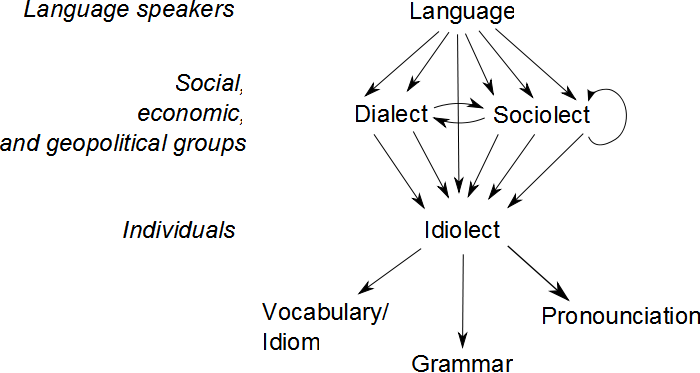
\includegraphics{http://adjectivespecies.com/wp-content/uploads/2012/04/language-hierarchy.png}
\caption{Language hierarchy}
\end{figure}

Put this way, we can come up with a sort of hierarchy of language. A
language is comprised of dialects and sociolects, subsets of the overall
language based around social, economic, or geopolitical groups. The
dialects and sociolects, in turn, are made up of the individial
idiolects of their members. There, of course, some mixing due to new
speakers of the language and borrowed terms, but also due to the fact
that individuals often belong to more than one social group, and thus
may take part in more than one sociolect or dialect - my partner is a
machinist, but he is also a furry, for instance. A good example might be
the apparent dichotomy between ``realistic'' and ``toony'' furry art,
perhaps due to the overlap between the furry subculture and the art
world (whereas ``realism'' isn't something I hear much at my own job as
a programmer).

Much of this focus on our means of communication ties into the Internet
and the prominence of its role within the fandom. There's really no
doubting that a good portion of the fandom ``grew up'' on the net. The
ways in which it facilitates communication between individuals or groups
regardless of geographic location fits in so well with a fandom that
bases so much of its existence around social interaction. There are a
few terms that become important due to this fact, namely ``text'',
``corpus'', ``medium'', and ``modality''. A ``text'' is a unit of
communication, whether it's a journal post, an image and all of its
associated discussion, such as comments, or a webpage like this. A
``corpus'' is a collection of related texts - this post would be a text,
but {[}adjective{]}{[}species{]} would be a corpus - though it can be
taken in broader terms, such as the collection of all different texts on
FurAffinity - images, journals, comments, user pages - or simply the
collection of all texts within our subculture: the furry corpus, if you
will.

``Medium'' and ``modality'' are similarly intertwined. The ``medium''
is, obviously enough, the way in which a text reaches us, and the
``modality'' is what the text is constructed of. For instance, words and
language would be the modality, whereas that can be divided into written
words read off a screen on a webpage, or spoken words shared among a
group of friends at a convention. The reason I'm bringing up these terms
is that, taken together, they form our social interaction within the
fandom, and the reason that it's \emph{important} is because, in
particular, our choices of media and corpi are language in and of
themselves: that is, that we rely on the Internet for so much of our
communication, whether out of necessity or desire, and allow the
idiolects that we've formed on the 'net to creep into our verbal
communications with each other is something of a statement in and of
itself.

Put another way, our medium is important because it involves the
concepts of human-computer interaction (HCI) and computer (or, more
specifically, Internet) mediated communication (IMC). The first, HCI, is
important because computers are not free-form entities through which we
may communicate however we want. Instead, we communicate through the
specific media of SecondLife, through comments on submissions on FA,
through MUCKs, MUDs, IRC, and IMs. The actual means of intereaction
within each is different from each other, and certainly different than
other media. For instance, posing actions, and thus role-playing, are
quite simple on MU*s and IRC, and thus more common, whereas the same is
not true of instant messages and the less-immediate form of comment
threads and forums. The latter concept of IMC becomes particularly
evident in SecondLife, where the action taken by your character on the
screen is distanced from reality by necessity. Shooting a gun, turning a
cartwheel, or doing a dance are all usually thought of physical
activities offline, but on SecondLife, they are all the result of
commands typed in by the user or accessed via the mouse on a head up
display.

It's an easy thing to say that communication is the basis of our
subculture, but more difficult to express it in terms of the source and
result of a sociolect comprised of the colliding idiolects of its
members. While that is far from the only thing that furry has going for
it, it's a definite signifier of our being a society in our own right,
and one of the easiest to perceive, once one takes a step back. We have
settled our concentration certain media for a variety of reasons - the
ease of constructing an avatar on the Internet, the mediated sharing of
texts through different websites and services, and the 'net's way of
connecting individuals across distance. Our choice of media is a form of
communication in a way, though not simply due to the benefits to be
gained from it. There is more, though, to be sure.

\subsubsection{On Semiotics}\label{on-semiotics}

When I first heard about the Sapir-Whorf Hypothesis, I rejected it
immediately. It states, in brief, that the way we conceive of the world
around us, the way we assign meaning to things, is shaped entirely by
the language that we use to describe that meaning. I think that part of
the reason that I had such a negative reaction to the idea right off the
bat was that I learned about the hypothesis via the constructed language
lojban. The idea behind lojban (always written with a lower-case `l') is
that, if the way we think is shaped by the language we use, than a
language that is totally and completely ``logical'' ought to help one to
think totally and completely logically.

That idea really grated on me for a few reasons. First of all, I was in
a Madrigal choir at the time, and while the Madrigal came from the
Renaissance period, much of the words to the songs spend time evoking
romantic imagery. That, and much of the songs we performed weren't
exactly Madrigals in their own right, but composed later in the Romantic
or Neo-romantic eras. Put simply, I was a teenager inundated in
romanticism - the concept of being able to explain everything only with
logical terms and without the metaphor inherent in romanticism didn't
jive with me. Additionally, having been brought up by two atheist
parents, I was going through my own spiritual renaissance at the time,
and so I was always finding these neat, non-spatiotemporal, sometimes
ineffible ideas around myself, whether it be religion or something more
new-agey.

I was a non-Whorfian, basically. I believed, at the time, that we fit
words entirely to the meanings that exist independently of those words.
There is certainly an argument to be made for that, as well. We all, in
one way or another, are able to perceive what a ``tree'' is. There's a
way for us to scientifically define it, and there isn't necessarily a
way for us to claim that a tree is only a tree because we have all
conceived of the language for defining what a tree is.

I'm no longer fifteen, though, and things have changed. I have had my
own experience with the way that meaning comes to us through language or
signs of some sort, not least of all with my attempts at such things
with these articles. I think that I might now call myself a believer in
Moderate Whorfianism. In his book \emph{The Act of Writing}, Daniel
Chandler explains that many linguists would find extreme Whorfianism
hard to swallow, but may accept a weak version of it as defined in the
following way:

\begin{itemize}
\tightlist
\item
  the emphasis is on the potential for thinking to be `influenced'
  rather than unavoidably `determined' by language;
\item
  it is a two-way process, so that `the kind of language we use' is also
  influenced by `the way we see the world'
\item
  any influence is ascribed not to `Language' as such or to one language
  as compared with another, but to the use \emph{within a language} of
  one variety rather than another (typically a \emph{sociolect} - the
  language used primarily by members of a particular social group)
\item
  emphasis is given to the social context of language use rather than to
  purely linguistic considerations, such as the social pressure in
  particular contexts to use language in one way rather than
  another.{[}1{]}
\end{itemize}

This leads us to the next topic of discussion: semiotics. There is
argument as to whether or not linguistics is a subset of semiotics, or
vice versa. Whereas linguistics aims to tackle the use and meaning of
language, semiotics aims to tackle the use and language of meaning. They
are certainly closely related - given that language, written language
specifically, but also speech, provides a measureable, non-objective
metric to study, much of semiotics deals with the use of words within a
certain context to either ascribe or convey meaning, as well as the
additional meaning conveyed via word choice.

Beyond that, however, semiotics also takes into account such things as
the medium and modality of communication, regardless of whether it has
to do with words. Semiotics is just as comfortable looking at body
language and posture, meaning conveyed through the layout of a webpage,
or even additional meanings conveyed through art, which most definitely
has something to with our own subculture. That is, rather than focusing
on language itself, semiotics focuses on the meanings conveyed between
actors within a community. It is not that linguistics has nothing to do
with meaning, nor that it doesn't take the social context into account,
simply that that focusing specifically on those areas is the realm of
semiotics, instead.

The process of ascribing meaning to a sign - be it a word, a gesture,
music, or some aspect of a piece of visual art - is known as semiosis.
Semiosis isn't something that happens on it's own, we don't ascribe
meaning to the word ``tree'' without having some framework in which to
ascribe that meaning. Signs are parts in the whole of sign systems or
``codes''. A code could be a language, but using that word in particular
is a poor choice, because language always takes place within some
context and carries additional signifiers along with it. ``Tree'' said
calmly, for instance, carries different connotations than ``TREE!''
shouted fearfully. Even in a text-only environment such as this, the
punctuation and capitalization are signs in and of themselves. All of
this is taking place within a cultural context, as well. With language
in particular, the sign (a word) is a portion of a code that is shared
among actors in a community, whether it's the community of
English-speakers (a language) or the community of people interested in
anthropomorphics interacting online (the sociolect of furries on the
Internet).

This all goes to show that semiotics goes beyond the individual. The
webcomic xkcd recently performed quite a feat{[}3{]} by displaying a
different comic to different viewers. The comic that was chosen depended
not only on the viewer's choice of browser, but also on their location
and even the size of their browser window. The title of the comic was
``Umwelt'', which is the collection of sign-relations (briefly, the pair
of sign-meaning, or the triad of sign-interpretant-meaning) that make up
one's perception of the world. We cannot help to do anything outside our
umwelt, other than to assimilate new meanings into it through semiosis.

We aren't nearly so solipsistic, though, and so every time our umwelt
collides with another through interpersonal relationships, we influence
each other. When umwelten group together naturally through an attractor
such as a mutual interest, we wind up with a semiotic niche. That is,
when a social group forms, a sociolect can form with them due to the way
the group steers semiosis, the way it finds meaning.

These semiotic niches work much the same way as umwelten, in that they
can converge and share boundaries - they all, after all, take part in
the world of meaning around them, known as the semiosphere. That is,
something like furry will share its meaning not only with Internet
culture, but also western culture, anime culture to some extent, and, as
a whole, belongs to this whole perceived world around us. Beyond the
semiosphere, ``language not only does not function, it does not
exist.''{[}4{]} Without some framework for meaning, be it words, visual
art, music, or anything, there is only formless thought.

\begin{figure}[htbp]
\centering
\includegraphics{http://adjectivespecies.com/wp-content/uploads/2012/04/semiotic-hierarchy1.png}
\caption{Semiotic hierarchy}
\end{figure}

If we were to modify our language hierarchy to be about semiotics
(helpfully done in advance), it would look something like this, then.
Similar to the idea that languages are made up of sociolects and
dialects, which are in turn made up of idiolects, so too is the
semiosphere made up of semiotic niches, which are in turn made up of the
umwelten of individual members, the combined basis for creating meaning
in the world around us. This is, of course, a necessary gloss over the
field of semiotics, which is quite large. The goal of this article isn't
to go into commutation tests and syntactic analysis of furry works,
though, just to provide a groundwork of the concepts of language and
semiotics in the fandom.

It is within this construct of signs and meaning that we not only form
our ideas of what means ``tree'', what an image of a tree is and what it
represents, but what abstract concepts such as our subculture are and
what they're made up of. As individuals and members, or even as
outsiders looking in, we build the sign-relations, we come up with the
meaning of what is and is not furry, each to our own. It is where those
interpretations meet and generate a coherent idea of furry within more
than just the individual's point of view that we wind up with the furry
fandom itself.

\subsubsection{Tying it all together}\label{tying-it-all-together}

At some point, the furry fandom started to coalesce. Some would put it
in the 1980s - a reader and friend posits that the fandom really got
started September 1st, 1980 at Noreascon with Steve Gallacci{[}5{]} -
some would put it much, much earlier, and some perhaps later, into the
'90s when the Internet became truly accessible. For the sake of this
artcle and much of this site in general, we'd probably go with some time
in the mid to late '80s for the source of the fandom. This was the time
when the umwelten, the spheres of meaning for individuals, began to
collide in enough numbers to form that critical mass that led to the
formation of a subculture rather than a collection of enthusiasts.
Furries doubtless existed before, as is certainly evident even within
our own readership, but the furry fandom as a culture phenomenon, the
basis of study for much of this site (rather than individual furries
themselves), relied upon this interest being actively shared among
ur-members.

It was a sort of participatory semiosis that helps to define the
exploratory beginnings of any new social group. It wasn't so much that
individuals hadn't come up with the idea of fox-people before, as that
now they were in the process of finding meaning in the fact that there
was a cultural identity to be had, and assigning it to the signs of
``funny animal'' and furry, to foxes and cats leading extraordinary or
banal lives, to the very feeling of membership. In her book
\emph{Straight}, Hanne Blank makes a similar argument that the growth of
heterosexuality (and its complement, homosexuality) was due in part to
the process of self identificiation, the semiosis among individuals that
reached a critical mass after a few influential authors such as Freud
became widely read.

In short, I tend to focus on what I'm calling the ``contiguous fandom''.
That is, a fandom made of of members which share the borders of their
umwelten, the meanings attached to the sign that is `furry', in order to
create a coherent whole of a fandom. This is the importance of
membership; it is the act of being actors in a community that helps to
define the community as an entity.

Another way to think of it is that this is our participation mystique.
By basing part of one's identity on one's membership to an idea or
community, one helps to define both oneself and the thing of which one
is a member. To put it in the terms of linguistics above, we readily
adopt our sociolect. Remember here that we're taking into account all of
the signs available to us. Not only are we taking in this social
interaction using words in a furry context, but we're always taking in
the visual aspect of furry art and the participatory aspect of
conventions, fursuiting, and so on.

Beyond just adopting the sociolect, however, we're continuously adding
to it. We aren't just passive observers, but we are actively
participating in the creation of new texts, whether it's voicing our
appreciation of art, taking part in role-playing, or even running a
silly meta-furry blog where one talks about the semiotics of the furry
subculture.

Given the contiguous fandom, I can't continue without providing some
thoughs on what's ``outside'' that mostly coherent group of individuals
that make up furry. There is also importance in not being a member, in
not having that participation mystique. When it comes to signs in
semiotics, there is a loose division into dyadic and triadic signs. With
dyadic signs, you simply have one entity assigning the meaning of what a
tree is to the sign ``tree'', but in triadic signs, one has the
additional context of just who it is that is doing the assigning
alongside what is is that is being assigned. This is the interpretant
sign the one to whom ``I'' and ``you'' hold meaning as opposed to one
and the other, and, although it's abstract, it becomes very important
when it comes to membership.

When someone says ``I am a furry'', they are using a dyadic sign to
signify that a portion of themselves is defined as a member of the furry
community. However, when someone says ``that person is a furry'', then
the sign shifts to being triadic: the interpretant is taking an active
role in specifying that a sign (``furry'') signifies an object (``that
person''). Someone can always construct their own sign relations at any
time, but when it involves a third party, it has the tendency of
muddying the waters of the semiotic niche (after all, if it were
straight-forward, there wouldn't be much discussion to have).

What this means is that someone can certainly contribute to the
sociolect without necessarily becoming a member of the society which
owns it. There are more than enough examples of this to go around:
\emph{Watership Down} and ``Robin Hood'', or perhaps Coyote or Raven or
Jackal. The creators of these signs and contexts did not necessarily
take up membership in the furry social group, but they certainly did add
to the niche of language and meaning that has been carved out over the
last thirty years or so. This is complicated even further by the fact
that the niche is made up of a community of actors rather than just one:
something like Coyote as trickster may seem plenty furry to one member
of the community, but only tangentially so, if at all, to another.

There are a few problems surrounding this concept of furry as a semiotic
niche, and they have to do with the depth at which one analyzes the
fandom, or the distance from it one stands. If, for example, one were to
step back from furry a little ways, one can look at it a different way
and see it in the context of a related field: genre theory.

Furry as a genre is, on the surface, not a surprising concept. One can
think of furry literature just as easily as one considers fantasy
literature, or perhaps historical fiction. There is an underlying topic
that lays beneath the corpi of all three genres. However, as Chandler
puts it, ``The classification and hierarchical taxonomy of genres is not
a neutral and `objective' procedure.''{[}6{]} The important point here
is that the difference between objective and subjective interpretation
is, in the terms of semiotics, the act of subjective interpretation is a
sign in and of itself. That so many furries today would consider
Disney's ``Robin Hood'' to be a furry movie holds meaning both in
regards to the object of the film and the fuzzy interpretants
themselves. It is difficult even for me to interpret the movie outside
of a furry context - I saw it first in Elementary school, and even then
spent time drawing foxes afterwards. Needless to say, genre's a
difficult thing to determine from within.

This leads us to the second issue of determining a definition from
within or without. If we bring back the concept of Moderate Whorfianism,
this becomes more evident. In that context, language influences
thinking, but if the thinking is the process of defining either one's
membership within the community, or, more dangerously, defining the
community as a whole as we are here, then a feedback loop is started. If
our contributions to the sociolect modify the sociolect that we're in
the process of studying, even individually, then it becomes even more
difficult to pin down. This is quite the problem when studying the
fandom from within.

Studying the fandom from outside introduces other related risks,
however. It's difficult to study something like this from the outside,
as well, without having some concept of the use of the texts involved
within their context. That is, it seems like studying a participatory
corpus such as that of the output of our subculture without
participating as well has the risk of coming up with an incomplete
mental map of what all is going on. A good example of this (and I do
mean good - the studies are well worth reading) would be the work of
Kathleen Gerbasi, such as her study Furries A to Z (Anthropomoprhism to
Zoomorphism){[}7{]}. While the study is well conducted and provides a
good, in-depth look at the fandom, entries to her livejournal page
indicate an involvement with the fandom not quite at the level of
membership, but perhaps above simple scientific observation.

There is, it seems, a bit of indeterminacy when it comes to studying
something such as a social phenomenon. By investigating or defining, we
change, or at least risk changing that which is investigated or defined.
It's part of the aforementioned feedback loop, as certainly the goal of
the investigator is to be changed in some way by the thing being
investigated. That's what gaining knowledge is all about.

Finally, the furry corpus in particular is extremely difficult to
analyze. This is mostly due to the proliferation of texts, media, and
modalities. We produce \emph{a lot}. It is to the point where it's even
difficult to break the corpus down beyond lines other than simply
different media. Even those lines are blurred by the profuse
cross-sharing of information across media, such as the reposting on
twitter of FA journals that link to one or several images, potentially
hosted on other sites.

There is, of course, plenty of writing to go by within the fandom. It's
not simply writing for the sake of adding to the furry genre, such as it
is, though, but writing in the form of image descriptions, journals, and
rants on twitter. The idea is carried further to social interaction with
written language, through twitter conversations, comments on images,
role-playing, and instant messaging. Beyond the word, however, there is
our focus on visual art; whether or not visual art is the primary draw
to the fandom is certainly up for debate, but there is a reason that one
of the primary social hubs online is an art website and one of the big
draws at conventions is the art-show and dealers den.

There are more complex forms of communication than static text and
images, though, and here is where things become quite difficult to
analyze in any meaningful way. Fursuits, for instance, provide
communication in a visual medium similar to that as art - they are
pleasing to look at and express the meaning of the character they are
intended to embody - but they are also an interactive medium. A medium
that can move and talk, can hug and bounce and stalk and take on a life
of its own.

And beyond even the concept of extending one's character into a costume
one can don, there is our social interaction that happens on a more
mundane basis, yet still within the boundaries of ``furry interaction''.
There is an acceptable behavior, however ill-defined, that goes along
with being a furry. It's difficult to speak of beyond tendancies and
social cues, as many such social customs that come with membership in a
subculture or fandom. It has been noted before, though, that one can
tell the furries at a furry convention and a furmeet apart from the
non-furs. There's a way that we act, which likely has much more to do
with the idea of shared membership and social status than an interest in
animals. JM, for instance, writes about the prevalence of geekiness and
the behavioral norms that go along with it as they pertain to our
fandom{[}8{]}.

There are subtle cues and portions of our sociolect all over the place,
though, and it doesn't always have to do with direct communication
between actors in the community. The subtler things such as structures
in websites (Flickr and DeviantArt, for instance, don't have a category
option specifically for species) and conventions (the previously
mentioned focus on dissemination of texts through the artshow and
dealers areas), or even in media already geared toward social
interaction such as MUCKs (again with a species flag) and SecondLife
(where one can purchase a skin not only of the species of one's
character, but of the exact color required).

Furry is a heady mix of a full slice of human society that somehow seems
to remain topical. We have the glue of our mutual interest in
anthropomorphics, but beyond that, we have spread our corpus across
several different texts in our own personal ways of generating meaning
within the context of our subculture. By the interaction of our own
spheres of meaning we have generated our own semiotic niche, however
fuzzy around the edges, and come up with this idea of ``furry''. There's
no real easy way to pull it apart, even given as broad a topic as
semiotics, but by investigating and participating, we always seem to
expand it all the further.

\subsubsection{Conclusion}\label{conclusion}

This thing we call ``furry'' is clearly more difficult to pin down than
one simple article or even a whole website will cover. It's something
that I'd tried before in a few different ways. In fact, it seems to be
something that everyone tries as part of their membership dues. Every
now and then, once a month or so, I'll come across a journal post of
someone else's take on the whole fandom, and the beautiful (and yes, a
little frustrating) part of it is that they're all totally different.

We can make at least one statement, having taken all of this into
account, though. Furry is a complex interaction of actors within a
social community surrounding an already complex sign-meaning
relationship. Beyond that, though, the issue grows complex by our
reliance on two main modalities: natural language, which is always prone
to misinterpretation; and visual art, which is only barely analyzable,
and limited further, anyhow, by the medium of primarily hand-drawn
images. Both of these are inherently ambiguous, and often based on
aesthetics and identification on a per-member basis. That is, what is
furry to one is not necessarily furry to another, or even the creator.
The final level of obfuscation comes through the means with which so
many interact with the fandom, via a willfully constructed avatar,
something which does not match the individual themselves out of
necessity.

This article and any like it will have it's necessary downsides. We
didn't really get anywhere, all told - we defined some terms in order to
help us understand the ways in which we interact with our subculture,
both throught the linguistic concept of a sociolect, a language used
among our co-fans, and the semiotic concept of a niche, a set of
meanings and sign relations shared by the members of the niche. It's
hard to get anywhere with either, though, especially in such a
loose-weaved community. Semiotics and lingustics are all about
statements of subtle facts made out in the open. There are concrete
tests and analyses to be done (if one could port the commutation test to
our visual art in order to find the ``graphemes'' of muzzles and tails,
that could lead to interesting results), but they're difficult to really
do well, and even if they were, it's not guaranteed that they would lead
to any results, nor if any of the results would even be welcome.

There are positives to be had as well, though. I hope that the article
has provided more insight into the the linguistics and semiotics of the
fandom. The ideas of sociolects and genres are a good way to think about
this broad base of which we are a part, because they provide a
foundation of words on which we can base our own explanations of what it
means to be a furry. And, beyond the definitions, it's nice to maintain
a certain sort of disputability. It allows for a greater membership
through greater self identification - more people can become furry
because the definition of what furry is can accomodate them. And hey,
that sense of mystery about the fandom is always nice, as well. It's a
hook for bringing in new members, and for
\href{http://adjectivespecies.com/2012/03/21/makyos-kaddish/}{keeping
the old ones interested}, too.

I know this has been a little out of the norm, but I wanted to actually
take my time to research an article and provide a more coherent look at
the reasons for studying the fandom, and for this site in general. These
things \emph{are} important to us, too. The meanings we create determine
our interactions within the fandom and how they take place. Beyond that,
though, by participating in our community as members, we contribute to
it. This is how we grow, explore, and find meaning,

Where to go from here? Well, I hope that the cognizance of the signs
around us is helpful in a way. Every word, every piece of art, and every
interaction between members is a sign from which we can glean a message
and to which we can attach our own individual meanings, however mundane.
The meanings inherent in these relations surround us and help define our
membership, and we're certainly always creating more. If nothing else,
there's always more work to go when it comes to exploring the furry
subculture.

\subsubsection{Citations}\label{citations}

{[}1{]} Chandler, Daniel. ``The Act of Writing''.
\url{http://www.aber.ac.uk/media/Documents/act/act.html} accessed April
3, 2012.

{[}2{]} Zik. ``furry lexicon''. \url{http://pastebin.com/GR7MqsnJ}
accessed, April 2, 2012.

{[}3{]} Munroe, Randall. ``Umwelt''. \url{http://xkcd.com/1037/}
accessed April 1, 2012.

{[}4{]} Lotman, Yuri M. On the semiosphere. (Translated by Wilma Clark)
Sign Systems Studies, 33.1 (2005).
\url{http://www.ut.ee/SOSE/sss/Lotman331.pdf} accessed April 5, 2012.

{[}5{]} Geddes, M." The History of the Furry Fandom, Pt 1" (2012).

{[}6{]} Chandler, Daniel. ``An Introduction to Genre Theory''.
\url{http://www.aber.ac.uk/media/Documents/intgenre/intgenre1.html}
accessed April 7, 2012.

{[}7{]} Gerbasi, Kathleen. ``Furries A to Z (Anthropomorphism to
Zoomorphism) in''Society and Animals``, 16, 197-222.
\url{http://www2.asanet.org/sectionanimals/articles/GerbasilFurries.pdf}
accessed March 15, 2012.

{[}8{]} JM. ``Geeks''.
\url{http://adjectivespecies.com/2012/04/09/geeks/} accessed April 9,
2012.
